\documentclass[a5paper]{book}

\usepackage[calc]{adjustbox}
\usepackage{lipsum}
\usepackage{wrapfig}
\usepackage{cutwin}
\usepackage{amsthm}
\usepackage{amsmath}
\usepackage{amssymb}
\usepackage{enumerate}
\usepackage{tikz}
\usetikzlibrary{calc,intersections,through,backgrounds}
\renewcommand*\rmdefault{dayroms}
\usepackage[T1]{fontenc}
\makeatletter
\renewcommand{\@chapapp}{Book}
\makeatother
\theoremstyle{plain}
\newtheorem{prop}{Proposition}
\renewcommand{\qedsymbol}{Q.E.D.}

\definecolor{blue}{rgb}{0.13, 0.67, 0.8}
\definecolor{yellow}{rgb}{1.0, 0.75, 0.0}
\definecolor{red}{rgb}{0.92, 0.3, 0.26}

\begin{document}
	

	\frontmatter
	\chapter{Preface}
	\mainmatter
	
		\chapter{}
		\centering\subsection*{DEFINITIONS.}
		\begin{enumerate}[I]
			\item A \textit{point} is that which has no parts.
			\item A \textit{line} is length without breadth.
			\item The extremities of a line are points. 
			\item A straight or right line is that which lies evenly between its extermities. 
			\item A surface is that which has length and breadth only. 
			\item The extremities of a surface are lines.
			\item A plane surface is that which lies evenly between its extremities. 
			\item A plane angle is the inclination of two lines to one another, in a plane, which meet together, but are not in the same direction. 
			\item A plane rectilinear angle is the inclination of two straight lines to one another, which meet together, but are not in the same straight line.
			\item When one straight line standing on another straight linem makes the adjacent angles equal, each of these angles is called a right angle, and each of these lines is said to be perpendicular to the other. 
			\item An obtuse angle is an angle greater than a right angle.
			\item An acute angle is an angle less than a right angle. 
			\item A term of boundary is the extremity of any thing. 
			\item A figure is a surface enclosed on all sides by a line or lines. 
			\item A circle is a plane figure, bounded by one continued line, called its circumference or periphery; and having a certain point within t, from which all straight lines drawn to its circumference are equal. 
			\item The point (from which the equal lines are drawn) is called the centre of the circle. 
			\item A diameter of a circle is a straight line drawn through the centre, terminating both ways in the circumference. 
			\item A semicircle is the figure contained by the diameter, and the part of the circle cut off by the diameter.
			\item A segment of a circle is a figure contained by a straight line, and the part of the circumference which cuts it off. 
			\item A figure contained by straight lines only, is called a rectilinear figure. 
			\item A triangle is a rectilinear figure enclosed by three sides. 
			\item A quadrilateral figure is one which is bounded by four sides. The straight lines and connecting the vertices of the opposite angles of a quadrilateral figure, are called its diagonals. 
			\item A polygon is a rectilinear figure bounded by more than four sides. 
			\item A traingle whose three sides are equal, is said to be equilateral. 
			\item A triangle which has only two sides equal is called an isosceles triangle. 
			\item A scalene triangle is one which has no two sides equal. 
			\item A right angled triangle is that which has a right angle. 
			\item An obtuse angled triangle is that which has an obtuse angle. 
			\item An acute angled triangle is that which has three acute angles. 
			\item Of four-sided figures, a square is that which has all its sides equal, and all its angles right angles. 
			\item A rhombus is that which has all its sides equal, but its angles are not right angles. 
			\item An oblong is that which has all its angles right angles, but has not all its sides equal. 
			\item A rhomboid is that which has its opposite sides equal to one another, but all its sides are not equal, nor its angles right angles. 
			\item All other quadrilateral figures are called trapeziums.
			\item Parallel straight lines are such as are in the same plane, and which being produced continually in both directions, would never meet. 
		\end{enumerate}
		\centering\subsection*{POSTULATES.}
		\begin{enumerate}[I]
			\item Let it be granted that a straight line may be drawn from any one point to any other point.
			\item Let it be granted that a finite straight line may be produced to any length in a straight line. 
			\item Let it be granted that a circle may be described with any centre at any distance from that centre. 
		\end{enumerate}
		
		\centering\subsection*{AXIOMS.}
		\begin{enumerate}[I]
		\item Magnitudes which are equal to the same are equal to each other. 
		\item If equals be added to equals the sums will be equal. 
		\item If equals be taken away from equals the remainders will be equal. 
		\item If equals be added to unequals the sums will be unequal. 
		\item If equals be taken away from unequals the remainders will be unequal. 
		\item The doubles of the same or equal magnitudes are equal. 
		\item The halves of the same or equal magnitudes are equal. 
		\item Magnitudes which coincide with one another, or exactly fill the same space, are equal. 
		\item The whole is greater than its part. 
		\item Two straight lines cannot include a space. 
		\item All right angles are equal. 
		\item If two straight lines () meet at a third straight lines () so as to make the two interior angles ( and ) on the same side less than two right angles, these two straight lines will meet if they be produced on that side on which the angles are less than two right angles. 
		\end{enumerate}
		\centering\subsection*{ELUCIDATIONS.}
		\newpage
		\centering\subsection*{PROPOSITIONS.}
		\begin{prop}
		

	
%			\begin{cutout}{1}{0.5\textwidth}{0pt}{2}
			On a given finite straight line (\tikz[baseline=-0.5ex]\draw[ultra thick] (0,0) -- (1,0);) to describe an equlateral triangle.\\
			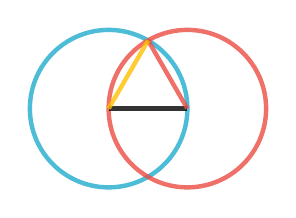
\begin{tikzpicture}[scale=1,opacity=0.8]
\coordinate (A) at (0,0);
\coordinate (B) at (1,0);
\draw[name path=C1,blue,ultra thick] (A) circle (1cm);
\draw[name path=C2,red,ultra thick] (B) circle (1cm);
\path [name intersections={of=C1 and C2}];
\coordinate (C) at (intersection-1);

\draw[ultra thick] (A) -- (B); 
\draw[ultra thick,red] (B) -- (C);
\draw[ultra thick,yellow] (C) -- (A);
\end{tikzpicture}
%			text
%		\end{cutout}
	\end{prop}

	
	\begin{proof}
		Describe 
			
\begin{tikzpicture}[scale=0.5,opacity=0.8,baseline=-0.5ex]
			\coordinate (A) at (0,0);
			\coordinate (B) at (1,0);
			\draw[name path=C1,blue,ultra thick] (A) circle (1cm);
			\draw[ultra thick] (A) -- (B); 
			\end{tikzpicture}
		 and 
	 		
\begin{tikzpicture}[scale=0.5,opacity=0.8,baseline=-0.5ex]
	 		\coordinate (A) at (0,0);
	 		\coordinate (B) at (1,0);
	 		\draw[name path=C2,red,ultra thick] (B) circle (1cm);
	 		\draw[ultra thick] (A) -- (B); 
	 		\end{tikzpicture}
 		 (postulate 3.); draw \tikz[baseline=-0.5ex]\draw[yellow,ultra thick] (0,0) -- (1,0); and \tikz[baseline=-0.5ex]\draw[red,ultra thick] (0,0) -- (1,0); (post. 1. ). then will 
	 	 		
\begin{tikzpicture}[baseline=-0.5ex,scale=0.5,opacity=0.8]
	 	 		\coordinate (A) at (0,0);
	 	 		\clip (-0.1,-0.1) rectangle (1.1,1.1);
	 	 		\coordinate (B) at (1,0);
	 	 		\path[name path=C1,blue,ultra thick] (A) circle (1cm);
	 	 		\path[name path=C2,red,ultra thick] (B) circle (1cm);
	 	 		\path [name intersections={of=C1 and C2}];
	 	 		\coordinate (C) at (intersection-1);
	 	 		\draw[ultra thick] (A) -- (B); 
	 	 		\draw[ultra thick,red] (B) -- (C);
	 	 		\draw[ultra thick,yellow] (C) -- (A);
	 	 		\end{tikzpicture}
		be equilateral. 
		\begin{align*}
			\text{For }  \tikz[baseline=-0.5ex]\draw[black,ultra thick] (0,0) -- (1,0); &= \tikz[baseline=-0.5ex]\draw[yellow,ultra thick] (0,0) -- (1,0);  \text{ (def. 15.)}\\
			\text{and  }\tikz[baseline=-0.5ex]\draw[black,ultra thick] (0,0) -- (1,0); &= \tikz[baseline=-0.5ex]\draw[red,ultra thick] (0,0) -- (1,0); \text{ (def 15.)} \\
			\therefore \tikz[baseline=-0.5ex]\draw[yellow,ultra thick] (0,0) -- (1,0); &= \tikz[baseline=-0.5ex]\draw[red,ultra thick] (0,0) -- (1,0); \text{ (axiom. 1.)} 
		\end{align*}



		
	\end{proof}
	

\end{document}